%%%%%%%%%%%%%%%%%%%%%%%%%%%%%%%%%%%%%%%%%%%%%%%%%%%%%%%%%%%%%%%%%%%%%%%%%%%%%%%
%%%%%%%%%%%%%%%%%%%%%%%%%%%%%%%%%%%%%%%%%%%%%%%%%%%%%%%%%%%%%%%%%%%%%%%%%%%%%%%
% %
% Title: Automatically generated Template for Dagstuhl Reports %
% Script used: abstracts-listing_tex.wml %
% originally developped by Tobias Maurer %
% 2005-02-15: Layout Template (by Jutta Huhse) %
% 2011-02-28: Layout adapted to Dagstuhl Reports (by Marc Herbstritt) %
% %
%%%%%%%%%%%%%%%%%%%%%%%%%%%%%%%%%%%%%%%%%%%%%%%%%%%%%%%%%%%%%%%%%%%%%%%%%%%%%%%
%
% This document requires the Dagstuhl Reports LaTeX style package dagrep.cls
% and corresponding graphic files.
% It can be downloaded from the following URL:
%
% http://www.dagstuhl.de/???
%
%%%%%%%%%%%%%%%%%%%%%%%%%%% head declarations %%%%%%%%%%%%%%%%%%%%%%%%%%%%%%%%%
%%%%%%%%%%%%%%%%%%%%%%%%%%%%%%%%%%%%%%%%%%%%%%%%%%%%%%%%%%%%%%%%%%%%%%%%%%%%%%%


%This is a template for producing reports for "Dagstuhl Reports".
%See dagrep.pdf for further information.

\documentclass[a4paper,UKenglish]{dagrep}
  %for A4 paper format use option "a4paper", for US-letter use option "letterpaper"
  %for british hyphenation rules use option "UKenglish", for american hyphenation rules use option "USenglish"
  %for section-numbered lemmas etc., use "numberwithinsect"

\usepackage{xspace}
%\usepackage{todonotes}
\usepackage{microtype}%if unwanted, comment out or use option "draft"
\usepackage{url}
% ============================================================
%:Markup macros for proof-reading
\usepackage{ifthen}
\usepackage[normalem]{ulem} % for \sout
\usepackage{xcolor}
\newcommand{\ra}{$\rightarrow$}
\newboolean{showedits}
\setboolean{showedits}{true} % toggle to show or hide edits
%\setboolean{showedits}{false} % toggle to show or hide edits
\ifthenelse{\boolean{showedits}}
{
	\newcommand{\meh}[1]{\textcolor{red}{\uwave{#1}}} % please rephrase
	\newcommand{\ins}[1]{\textcolor{blue}{\uline{#1}}} % please insert
	\newcommand{\del}[1]{\textcolor{red}{\sout{#1}}} % please delete
	\newcommand{\chg}[2]{\textcolor{red}{\sout{#1}}{\ra}\textcolor{blue}{\uline{#2}}} % please change
	\newcommand{\nbe}[3]{
		{\colorbox{#3}{\bfseries\sffamily\scriptsize\textcolor{white}{#1}}}
		{\textcolor{#3}{\sf\small$\blacktriangleright$\textit{#2}$\blacktriangleleft$}}}
}{
	\newcommand{\meh}[1]{#1} % please rephrase
	\newcommand{\ins}[1]{#1} % please insert
	\newcommand{\del}[1]{} % please delete
	\newcommand{\chg}[2]{#2}
	\newcommand{\nbe}[3]{}
}
%
\newcommand\rA[1]{\nbe{Reviewer A}{#1}{cyan}}
\newcommand\rB[1]{\nbe{Reviewer B}{#1}{olive}}
\newcommand\rC[1]{\nbe{Reviewer C}{#1}{magenta}}
\newcommand\ANS[1]{\nbe{Response}{#1}{teal}}
% ============================================================
%:Box comments/edits
\usepackage[most]{tcolorbox}
\ifthenelse{\boolean{showedits}}
{
  \newtcolorbox{inserted}{%
       title=Inserted text:,
       colframe=blue,colback=blue!5!white,
       breakable,
       leftrule=0mm, 
       bottomrule=0mm,
       rightrule=0mm,
       toprule=0mm,
       arc=0mm, outer arc=0mm,
       oversize
  }
  \newtcolorbox{deleted}{%
       title=Deleted text:,
       colframe=red,colback=red!5!white,
       breakable,
       leftrule=0mm, 
       bottomrule=0mm,
       rightrule=0mm,
       toprule=0mm,
       arc=0mm, outer arc=0mm,
       oversize
  }
  \newtcolorbox{refactored}{%
       % title=Heavily modifed/refactored text:,
       title=Rewritten text:,
       colframe=blue,colback=red!5!white,
       breakable,
       leftrule=0mm, 
       bottomrule=0mm,
       rightrule=0mm,
       toprule=0mm,
       arc=0mm, outer arc=0mm,
       oversize
  }
}{
  \newenvironment{inserted}{}{}
  %\newenvironment{deleted}{ \begin{comment} }{ \end{comment} }
  \let\deleted\comment
  \newenvironment{refactored}{}{} 
}
% ============================================================
%:Put edit comments in a really ugly standout display
%\usepackage{ifthen}
\usepackage{amssymb}
\newboolean{showcomments}
\setboolean{showcomments}{true}
%\setboolean{showcomments}{false}
\newcommand{\id}[1]{$-$Id: scgPaper.tex 32478 2010-04-29 09:11:32Z oscar $-$}
\newcommand{\yellowbox}[1]{\fcolorbox{gray}{yellow}{\bfseries\sffamily\scriptsize#1}}
\newcommand{\triangles}[1]{{\sf\small$\blacktriangleright$\textit{#1}$\blacktriangleleft$}}
\ifthenelse{\boolean{showcomments}}
%{\newcommand{\nb}[2]{{\yellowbox{#1}\triangles{#2}}}
{\newcommand{\nbc}[3]{
 {\colorbox{#3}{\bfseries\sffamily\scriptsize\textcolor{white}{#1}}}
 {\textcolor{#3}{\sf\small$\blacktriangleright$\textit{#2}$\blacktriangleleft$}}}
 \newcommand{\version}{\emph{\scriptsize\id}}}
{\newcommand{\nbc}[3]{}
 \newcommand{\version}{}}
\newcommand{\nb}[2]{\nbc{#1}{#2}{orange}}
\newcommand{\here}{\yellowbox{$\Rightarrow$ CONTINUE HERE $\Leftarrow$}}
\newcommand\rev[2]{\nb{TODO (rev #1)}{#2}} % reviewer comments
\newcommand\fix[1]{\nb{FIX}{#1}}
\newcommand\todo[1]{\nb{TO DO}{#1}}
\newcommand\on[1]{\nbc{Oscar}{#1}{olive}} % add more author macros here
\newcommand\jv[1]{\nbc{Jurgen}{#1}{red}}
\newcommand\cg[1]{\nbc{Carol}{#1}{blue}}
\newcommand\jh[1]{\nbc{James}{#1}{brown}}
\newcommand\ck[1]{\nbc{Claude}{#1}{cyan}}
   \definecolor{darkgreen}{rgb}{0,0.6,0}
\newcommand\katznote[1]{\nbc{Dan}{#1}{darkgreen}} % add more author macros here

%\newcommand\XXX[1]{\nbc{XXX}{#1}{darkgray}}
%\newcommand\XXX[1]{\nbc{XXX}{#1}{gray}}
%\newcommand\XXX[1]{\nbc{XXX}{#1}{magenta}}
%\newcommand\XXX[1]{\nbc{XXX}{#1}{olive}}
%\newcommand\XXX[1]{\nbc{XXX}{#1}{orange}}
%\newcommand\XXX[1]{\nbc{XXX}{#1}{purple}}
%\newcommand\XXX[1]{\nbc{XXX}{#1}{red}}
%\newcommand\XXX[1]{\nbc{XXX}{#1}{teal}}
%\newcommand\XXX[1]{\nbc{XXX}{#1}{violet}}
% ============================================================


\bibliographystyle{plain}%the recommended bibstyle

% Preamble with header information
\subject{Report from Dagstuhl Seminar 16252}
\title{Perspectives Workshop: Engineering Academic Software}
\titlerunning{16252 --- Perspectives Workshop: Engineering Academic Software}%optional

% PLEASE DON'T PUT EMAILS IN PUBLIC DOCUMENTS! (ON)

\author[1]{Carole Goble}
  \affil[1]{University of Manchester, England --- \url{http://www.manchester.ac.uk/research/Carole.goble/}}
  % \url{mailto:carole.goble@manchester.ac.uk}}

\author[2]{James Howison}
  \affil[2]{The University of Texas at Austin, USA ---  \url{https://www.ischool.utexas.edu/people/person_details?PersonID=175}}
  % \url{mailto:jhowison@ischool.utexas.edu}}

\author[3]{Claude Kirchner}
  \affil[3]{Inria, France --- \url{http://www.loria.fr/~ckirchne/}}
  % \url{mailto:claude.kirchner@inria.fr}}

\author[4]{Oscar Nierstrasz}
  \affil[4]{University of Bern, Switzerland --- \url{http://scg.unibe.ch/staff/oscar}}

\author[5]{Jurgen J. Vinju}
  \affil[5]{Centrum Wiskunde \& Informatica, The Netherlands --- \url{http://homepages.cwi.nl/~jurgenv}}
  % \url{mailto:Jurgen.Vinju@cwi.nl}}

%Organizer macros:%%%%%%%%%%%%%%%%%%%%%%%%%%%%%%%%%%%%%%%%%%%%%%%%%%%%%
\seminarnumber{16252}
\semdata{\emph{20}.--\emph{24}.~\emph{June}, \emph{2016} --- \url{http://www.dagstuhl.de/16252}}
\subjclass{\emph{D.0. Software General}, \emph{}} % Cite, e.g., as B.3.3 Performance Analysis and Design Aids.} %mandatory
\keywords{\emph{Scientific Software, Data Science, Software Engineering}} % mandatory
% \additionaleditors{Tom Collector} %optional
%%%%%%%%%%%%%%%%%%%%%%%%%%%%%%%%%%%%%%%%%%%%%%%%%%%%%%%%%%%%%%%%%%%%%%%

%Dagstuhl editorial office macros:%%%%%%%%%%%%%%%%%%%%%%%%%%%%%%%%%%%%%
\volumeinfo%(easychair interface)
  {Carole Goble, James Howison,  Claude Kirchner, Oscar Nierstrasz, Jurgen Vinju}%editor names
  {5}%number of editors
  {Perspectives Workshop: Engineering Academic Software}%seminar title
  {1}%volume
  {1}%issue
  {1}%starting page number
\DOI{10.5362/DagRep.1.1.1}%(DagRep.<volume no>.<issue no>.<firstpage>)
%%%%%%%%%%%%%%%%%%%%%%%%%%%%%%%%%%%%%%%%%%%%%%%%%%%%%%%%%%%%%%%%%%%%%%%
% ============================================================
\newcommand{\ie}{\emph{i.e.},\xspace}
\newcommand{\eg}{\emph{e.g.},\xspace}
\newcommand{\etal}{\emph{et al.}\xspace}
\newcommand{\etc}{\emph{etc.}\xspace}
% ==========================================================

\begin{document}

\maketitle

%------------------------------------------------------------------------
%------------------------------------------------------------------------
% this is a standard text with some seminar specific information
\begin{abstract}

\end{abstract}
%------------------------------------------------------------------------

%% ==================================================
%\section*{About the edit macros}
%
%\on{Please use edit macros for comments you insert. See ``edit-macros.tex'' and add one for yourself if necessary.}
%
%There are generic macros for \todo{stuff to do} and \fix{stuff to fix}.
%
%There are macros for \ins{inserted text}, \del{deleted text}, and text to be changes \chg{from this}{to that}.
%
%
%\begin{inserted}
%There are also macros for blocks of text that have been inserted, deleted or refactored. These are useful to indicate proposals for changes to be checked by others in the pipeline.
%\end{inserted}

% ==================================================
\section{Executive Summary}
\summaryauthor[Carole Goble, James Howison,  Claude Kirchner, Oscar Nierstrasz, Jurgen Vinju]{Carole Goble, James Howison,  Claude Kirchner, Oscar Nierstrasz, Jurgen Vinju}

\license

This Dagstuhl Perspectives Workshop brought together activists, experts and stakeholders on the subject of high quality software produced in an academic context.\footnote{We include any software which is part of either research processes and/or output, while excluding more generic administrative software for research and education management.}
Our current dependence on software across the sciences is already significant, yet there are still more opportunities to be explored and risks to be overcome. The academic context is unique in terms of its personnel, its goals of exploring the unknown and its demands on quality assurance and reproducibility.

We refer to the IEEE Internet Computing article ``Better Software, Better Research''~\cite{Goble2014} which motivated the topic. In this workshop we took the following perspective of a research team which is in either or both of the following situations:
\begin{itemize}
\item consuming or producing software as \emph{an output} of the academic process;
\item consuming or producing software as \emph{a component} of the research methods;
\end{itemize}

Society is now in the tricky situation where several deeply established academic fields
(\eg physics, biology, mathematics) are shifting towards dependence on software, programming technology and software engineering methodology
which are backed only by young and rapidly evolving fields of research (computer science and software engineering).  Full accountability and even validity of software-based research results are now duly being challenged.

With the outputs of this interactive and productive perspectives workshop, we strive to contribute in a positive manner to the above challenges. We formulated taxonomies with definitions to clarify the domain, we co-authored concrete policy and process documents to improve the status and recognition of academic software development and academic software engineers, and finally we formulated a list of 18 concrete declarations of intent (``I will'' pledges). This list was presented to the WSSSPE community~\cite{wssspe_manifesto} to acquire feedback and it will be the backbone of the Dagstuhl Manifesto document we are editing. It serves to motivate change by proposing policy changes with concrete actions and instilling positive attitudes towards academic software.


\textbf{The participants of the workshop} came from three major groups. The first group consists of active and visible members of the \emph{global academic software engineering community}. They represent (formal) institutions such as the Software Sustainability Institute, the Software Carpentry Foundation, and eScience and data science centers from across the globe. The second group contributed researchers in \emph{empirical software engineering}, with a specific eye on studying the principles and practices of academic software engineering. The final group contributed \emph{researchers as an audience}: software engineering researchers with a long experience in engineering software for software itself or software for specific academic research fields.

We found that without exception the participants were motivated and able to actively contribute to the proceedings of the workshop; the mix of people proved to be well-balanced. This balance is an accomplishment, given that invitees from computer science were far more likely to know of Dagstuhl workshops than other groups. To attest to our outcomes we've selectively listed three (paraphrased) verbal statements here:
\begin{itemize}
\item ``The workshop was a transformational experience for me; I've learned an entire new perspective on my field and I intend to apply the insights in my daily practice.''
\item ``I had an epiphany yesterday after dinner; now I understand how to connect the data science research at my university to the computer science department.''
\item ``Before the workshop I had no idea so many initiatives were already underway in [improving] academic software engineering; this has given my understanding of the challenges a real boost and I know what the some of the next steps to take are.''
\end{itemize}

\textbf{The schedule of the workshop} was designed to maximize both interactive discussion and work towards tangible outputs. Key points were: to start the day with inspiring presentations to set the stage, then to have at least 40\% of the day time allocated to free discussion time, and to explicitly share successes (output) of each day's breakout groups in a plenary session.

The workshop started on Monday with a quick and tightly timed round of 2 minute personal introductions. Otherwise on Monday, Tuesday and Thursday the program was structured equally: in the morning we would have plenary presentations which included exploratory discussions. These sessions were meant to bring everybody up-to-speed with ongoing and past initiatives. During and after lunch we used a board with sticky notes to define break-out groups. Each break-out group was centred around a specific discussion topic and (usually) a specific idea for an output document was associated with it. After coffee we would go back to the same break-out group to collaboratively record the notes and lessons from each group (stored in a shared online document). Between 17:00 and 18:00 we reconvened and harvested the results of each breakout group with the others. People could and did freely switch between breakout groups but this was not a common thing.

On Wednesday we had an ``open-mic'' session with 8 presentations of around 10 minutes, sharing experiences and results, before we had a long walk in the surroundings. The organizers also designed an initial skeleton structure and ideas for the manifesto that day.

On Thursday afternoon and Friday morning we all worked together on our Dagstuhl Manifesto by first reworking our notes into the ideas around the manifesto, specifically a list of ``I will'' pledges with references and motivation. Finally, Friday afternoon a small remaining group re-ordered the group's manifesto notes into a well-structured list of 18 pledges. Two of the organizers remained to continue to edit the current report and the manifesto document.

\textbf{Output documents} of the workshop are organized under the ``dagstuhleas'' organisation on GitHub.\footnote{\url{https://github.com/dagstuhleas}} This currently features 6 draft documents, including the current report and (a) the manifesto, (b) the Research Software Engineering Handbook, (c) a Literature Survey, (d) a Taxonomy on Software Credit Roles, and (e) a Software Award Proposal. Next to these documents, an R\&D project proposal was produced on measuring the impact of academic software.

\textbf{The remainder of this document} summarizes the morning sessions by listing the abstracts of each talk, the afternoon breakouts by describing each topic and its results, and finally the research questions on the topic of engineering academic software we have collected.

\tableofcontents

% ==================================================
\section{Overview of Talks}

These are the talks presented in the morning sessions of workshop, chronologically ordered.

%-------------------------------------------------------
%\newpage

%------------------------------------------------------------------------
\abstracttitle{Sustainable Software for Science}
\abstractauthor[Daniel S. Katz]{Daniel S. Katz (University of Illinois at Urbana-Champaign, USA)}

Progress in scientific research depends on the quality and accessibility of research software at all levels. It is now critical to address many new challenges related to the development, deployment, maintenance, and sustainability of open-use research software: the software upon which specific research results rely.  \emph{Open-use software} means that the software is \emph{widely accessible} (whether open source, shareware, or commercial).  \emph{Research software} means that the choice of software is \emph{essential to specific research results}; using different software could produce different results.

In addition, it is essential that scientists, researchers, and students are able to learn and adopt a new set of software-related skills and methodologies. Established researchers are already acquiring some of these skills, and in particular, a specialized class of software developers is emerging in academic environments who are an integral and embedded part of successful research teams. WSSSPE\footnote{\url{http://wssspe.researchcomputing.org.uk}.} provides a forum for discussion of these challenges, including both positions and experiences, and a forum for the community to assemble and act.

This talk focused on the Third Workshop on Sustainable Software for Science: Practice and Experiences (WSSSPE3)~\cite{wssspe3}. It summarized the discussions, future steps, organization, and status of a set of self-organized working groups on topics including developing pathways to funding scientific software; constructing useful common metrics for crediting software stakeholders; identifying principles for sustainable software engineering design; reaching out to research software organizations around the world; and building communities for software sustainability. Some of these groups have executed these activities that they scheduled, some have in part, and others have not.  A point of discussion was why these groups came to these points, and how the WSSSPE community can encourage groups to act.

%------------------------------------------------------------------------
\abstracttitle{Supporting Research Software Engineering}
\abstractauthor[Mike Croucher]{Mike Croucher (University of Sheffield, UK)}

``Long Tail Science'' --- attributed to Jim Downing of the Unilever Centre for Molecular Informatics --- refers to the large number of small research units that perform a huge amount of research. Much of this research involves the generation of code by relatively untrained and inexperienced programmers.

In this talk, Croucher described the challenges of working as a Research Software Engineer who supports these programmers using the University of Sheffield as a case study and introduced the efforts to build a community (``a union'') of Research Software Engineers in the UK: \footnote{\url{http://www.rse.ac.uk/who.html}}.

%------------------------------------------------------------------------
\abstracttitle{Sustainability Design}
\abstractauthor[Christoph Becker]{Christoph Becker (University of Toronto, CA)}

Sustainability --- the ``capacity to endure'' --- has emerged as a challenge with transformative impact on many disciplines and professions, including software engineering. It requires simultaneous consideration of at least five dimensions: environmental resources, social and individual well-being, economic prosperity, and long-term technical viability. This requires a cross-disciplinary approach to research and design that moves beyond narrow-minded solutionism to emphasize an appreciation of ``wicked problems'' over a focus on puzzles and pieces; systems thinking over computational problem solving; and an integrated understanding of socio-technical systems. These shifts do not come easily, and for most systems, the hidden sustainability effects of past decisions in systems design are unknown. We can call this a system's ``sustainability debt''.

In this talk, Becker described how synergies across a range of disciplines united by the need for new design approaches focused on sustainability led to the Karlskrona Manifesto for Sustainability Design.\footnote{\url{http://www.sustainabilitydesign.org}}
He characterized principles of sustainability design and the key influence of requirements activities on the sustainability debt of a system under design. He presented recent efforts to develop this area of research, including an interview study of software professionals, as a starting point to a discussion of barriers and opportunities for sustainability design research.

%------------------------------------------------------------------------
\abstracttitle{What We Have Learned about Using Software Engineering Practices in Scientific Software}
\abstractauthor[Jeffrey Carver]{Jeffrey Carver (University of Alabama, USA)}

The increase in the importance of Scientific Software motivates the need to identify and understand which software engineering (SE) practices are appropriate. Because of the uniqueness of the scientific software domain, existing SE tools and techniques developed for the business/IT community are often not efficient or effective. Appropriate SE solutions must account for the salient characteristics of the scientific software development environment. To identify these solutions, members of the SE community must interact with members of the scientific software community. In this presentation, Carver discussed the findings from a series of case studies of scientific software projects, an ongoing workshop series, and interactions between his research group and scientific software projects.

%------------------------------------------------------------------------
\abstracttitle{Lessons from the YT project}
\abstractauthor[Matthew Turk]{Matthew Turk (University of Illinois Urbana-Champaign, USA)}

In this talk, Turk described the engineering practices, both social and
technical, around the YT project.\footnote{\url{http://yt-project.org}}
He described the positive aspects and the failure modes, and how the YT team attempted to
route around these failure modes.

%------------------------------------------------------------------------
\abstracttitle{Software as Academic Output}
\abstractauthor[Caroline Jay, Robert Haines]{Caroline Jay and Robert Haines (University of Manchester, UK)}

Software is now considered to be an output of academic research in its own right: venues such as SoftwareX and the Journal of Open Research Software highlight it as a primary contribution, and the UK Research Council includes a software category in the ResearchFish\footnote{\url{http://www.researchfish.com}} application used to collect the outcomes of research projects. This phenomenon is still fairly recent, however, and two questions arise when trying to determine the validity of --- or, arguably, requirement for --- software as a product of the research process: (i) when should it be considered an output, and (ii) what form should that output take?

To determine when software should be considered an output, we must consider its role in the research process. Is it a tool for supporting the work, or does it represent the research itself? To a computer scientist in the field of workflow management, the software would be considered a direct output, integral to the research. To a biologist, this same software would be considered a tool: useful for analyzing results, but not in itself an output of the research. For a bioinformatician both using and developing the tool, the answer is somewhere in the middle: whilst the core research may be in the life science domain, the modifications made to the tool as a result of this work could also be considered an output, advancing workflow management.

If the software is integral to the research --- and therefore a potential output --- what form should that output take? The FAIRDOM project\footnote{\url{http://fair-dom.org}} supports computational research that is FAIR: Findable, Accessible, Interoperable, Reusable. We suggest a modified version of these principles can be usefully applied to software too: it should be Findable, Accessible, Reusable and Extensible. To be findable, software must be searchable and discoverable by others, preferably via a persistent identifier. Accessible software can be viewed and downloaded by others. Reusable software can be re-run, potentially with other input data. Finally, Extensible software can be modified or extended to deal with new situations; to achieve this, the source code should be available.

The FARE principles are a starting point for defining best practice, or the ``gold standard'' for academic software outputs. An exemplar of the application of these principles is described in the authors' recent paper, ``ABC: Using Object Tracking to Automate Behavioural Coding''~\cite{apaolaza_2016}, published at the 2016 ACM CHI conference. The source code is openly available on GitHub, making it accessible and extensible, and both this and the software environment (in a Docker container), are identified by DOIs, making the software findable and reusable.

Following the FARE principles will help to ensure that software intended to be a primary output of research is fit for purpose. Applying them in any situation where software is developed as part of research --- whether it is considered a primary output or not --- is also recommended, to help ensure that the resulting research is robust and reproducible.

%------------------------------------------------------------------------
\abstracttitle{Software Heritage}
\abstractauthor[Claude Kirchner]{Claude Kirchner (INRIA, FR)}

%\jv{I wrote this, is it ok Claude?}
In this talk Kirchner introduced the \emph{Software Heritage} project\footnote{\url{http://www.softwareheritage.org}}, in the week just before its launch.
A quote from the web site explains the concept and the goals:
\begin{quote}
``Software Heritage collects and preserves software in source code form, because software embodies our technical and scientific knowledge and humanity cannot afford the risk of losing it.
Software is a precious part of our cultural heritage. We curate and make accessible all the software we collect, because only by sharing it can we guarantee its preservation in the very long term.''
\end{quote}

%------------------------------------------------------------------------
\abstracttitle{Software Metadata: Describing ``Dark Software'' in Geosciences}
\abstractauthor[Daniel Garijo]{Daniel Garijo (Technical University of Madrid, ES)}

In this talk Garijo provided an overview of the current state of the art for software description in Geosciences, along with an approach to facilitate this task in OntoSoft, a distributed semantic registry for scientific software. Three key aspects of OntoSoft are: a software metadata ontology designed for scientists, a distributed approach to software registries that targets communities of interest, and metadata crowdsourcing through access control. Software metadata is organized using the OntoSoft ontology, designed to support scientists to share, document, and reuse software, and organized along six dimensions: identify software, understand and assess software, execute software, get support for the software, do research with the software, and update the software.

%------------------------------------------------------------------------
\abstracttitle{Organising a Research Team around the Research Software around the Research Team in Software Engineering}
\abstractauthor[Jurgen J. Vinju]{Jurgen J. Vinju (Centrum Wiskunde \& Informatica, NL)}

Vinju's talk was about the motivation, experiences and lessons learned around the SWAT research group at CWI and its core product used for research and transfer, the meta-programming language and platform, Rascal,\footnote{\url{http://www.rascal-mpl.org}} which is hosted from the open-source organisation Use The Source.\footnote{\url{http://www.usethesource.io}}

%------------------------------------------------------------------------
\abstracttitle{Software Citation --- Principles, Discussion, and Metadata}
\abstractauthor[Daniel S. Katz]{Daniel S. Katz (University of Illinois at Urbana-Champaign, USA)}

Katz presented an overview of work done by the Force11 Software Citation Working Group\footnote{\url{https://www.force11.org/group/software-citation-working-group}}~\cite{10.7717/peerj-cs.86}.
This work includes rationales for citing software, information on the WSSSPE and Force11 groups involved in developing software citation principles, and the process used to develop them.
It also includes the six principles themselves:\begin{enumerate}
\item the importance of software,
\item the need to credit and attribute the contributions software makes to research,
\item to be able to uniquely identify the cited software software,
\item that the identifiers and metadata about software should be persistent,
\item that citations should enable access to the software and associated information about the software that informs its use,
and
\item that citations should facilitate identification of and access to the specific version of software that was used, such as by version number, revision numbers, or variants such as platforms.
\end{enumerate}
%
The talk also provided practical information on how to semi-automatically take code on GitHub and publish it on Zenodo, obtaining a DOI that can then be cited.\footnote{\url{https://guides.github.com/activities/citable-code/}}
Finally, the talk brought up a number of the ongoing discussions at the WSSSPE and Force11 working groups and their determinations, such as what software to cite, how to uniquely identify software, that peer-review of software is important but not required for citation, and how publishers can help.

%------------------------------------------------------------------------
\abstracttitle{Best Practices by Any Other Name}
\abstractauthor[Katie Kuksenok]{Katie Kuksenok (University of Washington --- Seattle, USA)}

% \jv{adapted from Alice's blog, ok Katie?}
This talk looked at intersections of the technical, social, and cognitive aspects of software engineering in research, and asked how the available community and skill resources could be leveraged. It brought together various elements raised throughout the workshop so far, including different roles that had been identified, the need for software engineers to learn from scientists just as we hope researchers learn software engineering practices, and overcoming communications barriers.

Katie also provided a link to a short blog post summary with figures.\footnote{Shortened URL to article at \url{https://medium.com/hci-design-at-uw}: \url{https://goo.gl/Lxqrt5}}

%------------------------------------------------------------------------
\abstracttitle{ASCL: Restoring Reproducibility --- Making Scientist Software Discoverable}
\abstractauthor[Alice Allen]{Alice Allen (University of Maryland --- College Park, USA)}

%\jv{adapted from your blog Alice, ok?}
%\meh{I presented an overview of the ASCL, its history and a few of the changes to our infrastructure, the lessons we learned from looking at what other astro code registries and repositories had done and what we did with those lessons, and some of the impact we have on the community.} \on{rambling sentence}

Allen presented an overview of the Astrophysics Source Code Library (ASCL)\footnote{\url{http://ascl.net}} and its history.
She also discussed a few of the changes to the ASCL infrastructure, lessons learned from looking at what other astro code registries and repositories had done, what ASCL did with those lessons, and some of the impact ASCL has had on the community.

%------------------------------------------------------------------------
\abstracttitle{A Short (and Probably Incomplete) History of Research Software Engineers in the UK}
\abstractauthor[Robert Haines]{Robert Haines (University of Manchester, UK)}

\begin{quote}
``\textit{Before software can be reusable it first has to be usable}'' --- Ralph Johnson, University of Illinois at Urbana-Champaign.
\end{quote}

A growing number of people in academia combine expertise in programming with an intricate understanding of research. Although this combination of skills is extremely valuable, these people lack a formal place in the academic system; they are not academics with a personal research agenda. This means there is no easy way to recognize their contribution, to reward them, or to represent their views.

One of the largest obstacles to overcome in recognizing this group of people is that they are often ``hiding'' in their institutions under a myriad different job titles and roles: Post-Doc, Research Associate, System Administrator, Computer Officer, and so on. In the instance of Post-Docs and Research Associates it is often the case that these people suddenly find that they have written too much code, and not enough papers, and so they fall foul of the usual metrics used to evaluate them for promotion. Being the person in the lab who ``knows about computers'' can be detrimental to your career.

These topics came up frequently at the Software Sustainability Institute's Collaborations Workshop in 2012. At this ``unconference'' style event a number of us repeatedly found ourselves in sessions discussing career paths, credit, recognition, metrics and reward, for those of us working in academia, who weren't academics. Without a name, it is difficult for people to rally around a cause, so we created the term Research Software Engineer (RSE) to describe the intersection of ``The Craftsperson and the Scholar''.\footnote{\url{http://www.software.ac.uk/blog/2012-11-09-craftsperson-and-scholar}}
RSEs are facilitative, supportive and collaborative; part of the academic community and its institutional memory, providing continuity and stability for its academic software. We also created the UK Community of Research Software Engineers\footnote{\url{http://www.rse.ac.uk/}} (UKRSE) as a focal point for our future campaigns and the Institute made the promotion of the RSE job role a cornerstone of their policy, lobbying the UK Government and Research Councils for RSEs to be recognized at a high level.

Since 2012 the RSE job role has gained traction in a number of institutions and has been endorsed by the Engineering and Physical Sciences Research Council in the UK (EPSRC). There are groups employing RSEs in University College London, the University of Manchester, the University of Cambridge, the University of Southampton and the University of Sheffield, with more in the process of being set up all the time. The EPSRC has funded seven RSE Fellowships, who have a remit to develop and support software and users of software, and has also funded a network of RSE leaders\footnote{\url{http://gow.epsrc.ac.uk/NGBOViewGrant.aspx?GrantRef=EP/N028902/1}} to further build the community of RSEs and develop the next round of Fellowships.

This year we held the world's first RSE Conference in Manchester, UK\footnote{\url{https://www.software.ac.uk/blog/2016-10-04-future-rses-looking-rosy-following-phenomenal-conference}}. It was the first conference to focus on the practice of rsearch software engineering and included sessions on the issues that affect people who write and use software in research as well as presented talks and workshops where new tools and techniques were taught. The conference attracted over 200 people from 14 countries, so we look forward to further expanding our community and building links with colleagues all over the world in the near future.

%------------------------------------------------------------------------
\abstracttitle{101companies --- Making a Failing Project Succeed}
\abstractauthor[Ralf L\"ammel]{Ralf L\"ammel (Universit\"{a}t Koblenz-Landau, Germany)}

% \jv{Ralf, I adapted this from Alice's blog, ok?}
L\"ammel presented the 101Companies project: a software \emph{chrestomathy}, from ``chresto'', meaning ``useful'' and ``mathein'', meaning ``to learn.'' 101 is a knowledge resource for technological space travel (between all kinds of technological spaces). It can serve to compare technologies, for programming education, and can serve as a playground for student projects. L\"ammel discussed some of the challenges the project is experiencing and some of the ways in which it is succeeding.

%------------------------------------------------------------------------
\abstracttitle{UE eScience Institute Initiatives}
\abstractauthor[Cecilia Aragon]{Cecilia Aragon (University of Washington -- Seattle, USA)}

Thanks in part to the recent popularity of the buzzword ``big data,'' it is now generally understood that many important scientific breakthroughs are made by interdisciplinary collaborations of scientists working in geographically distributed locations, producing and analyzing vast and complex data sets. The extraordinary advances in our ability to acquire and generate data in physical, biological, and social sciences are transforming the fundamental nature of science discovery across domains. Much of the research in this area, which has become known as data science or eScience, has focused on automated methods of analyzing data such as machine learning and new database techniques. Less attention has been directed to the human aspects of data science, including how to build interactive tools that maximize scientific creativity and human insight, and how to train, support, motivate, and retain the individuals with the necessary skills to produce the next generation of scientific discoveries.

In this talk, Aragon discussed the history and ongoing initiatives at the UW eScience Institute, including opportunities to participate in the \$37.8M Moore/Sloan Data Science Environment at UW, UCB, and NYU, and speculate upon future directions for data science. In particular, she discussed new initiatives at UW such as the eScience Incubator and the Data Science for Social Good program and focused on results of ethnographic studies of their projects and future work in the Data Science Studies working group. She further argued for the importance of a human-centered approach to data science as necessary for the success of 21st century scientific discovery. She attested that we need to go beyond well-designed user interfaces for data science software tools to consider the entire ecosystem of software development and use: we need to study scientific collaborations interacting with technology as socio-technical systems, where both computer science and social science approaches are interwoven.

%------------------------------------------------------------------------
\abstracttitle{The Netherlands eScience Center}
\abstractauthor[Rob van Nieuwpoort]{Rob van Nieuwpoort (The Netherlands eScience Center (NLeSC), NL)}

The Netherlands eScience Center (NLeSC) is the Dutch national hub for
the development and application of domain overarching software and
methods for the scientific community. NLeSC develops crucial bridges
between increasingly complex modern e-infrastructures and the growing
demands and ambitions of scientists from across all disciplines. The
application of digitally enhanced scientific practices makes sure that
returns can be achieved from scientific investments. In support of this
goal NLeSC funds and simultaneously funds and participates in
multidisciplinary projects, with academia and industry, with optimized
data-handling, efficient computing and big-data analytics at their
core.

NLeSC contributes exclusively to multidisciplinary projects with the
potential to deliver scientific excellence, in terms of breakthroughs
and in the realization of unique eScience methodologies. Many
organizational practices, such as our open call strategy and other
funding models ensure that new projects fulfill these criteria.

Apart from contributions to scientific publications in high-impact
scientific journals and conferences, NLeSC's primary deliverables are
eScience instruments (\eg software tools, workflows). Whilst the
instruments may include a domain specific component, primarily these
tools overarch multiple domains. The instruments are efficient,
calibrated, reliable and accessible, and based on excellent standards
of code quality utilizing meta-data standards and software development
environments. Successful instruments are made publicly available as
part of NLeSC's eScience technology platform (eStep) program. This
platform provides easy access to the developed tools and instruments
to the broader scientific community and industry alike. NLeSC also
shares non-scientific technical results, documentation and best
practices in the knowledge base that also is a part of eStep.

NLeSC also plays a key role in optimizing and disseminating the best
practices in the areas of software sustainability and
data-stewardship, including the need to engage with communities of
practices, data-publishers and related initiatives.

The rapid growth of data and computing initiatives risks unnecessary
fragmentation and duplication. NLeSC works with numerous partner
organizations, nationally and internationally, to identify common
challenges such as training and career support for eScientists, as
well as providing thought leadership on issues such as
data-stewardship and software sustainability. NLeSC is a joint
initiative of the Dutch national research council (NWO) and the Dutch
organization for ICT in education and research (SURF).



%\license
%\jointwork{Bry, Fran\c{c}ois;}
%\abstractref[]{} % [] --- URL, {} --- reference description (a la thebibliography)
%\abstractrefurl{} % preferrably DOI-based URL

%------------------------------------------------------------------------
\abstracttitle{On ImpactStory, Scientific Software Map, and depsy}
\abstractauthor[James Howison]{James Howison (University of Texas -- Austin, USA)}

There is a need to provide insights into the scientific software ecosystem~\cite{bogart_mapping_2015}: the set of projects, their software products, their authors, their dependencies, the papers describing them, and papers that have used the software to undertake science.  Such insights are useful for many players in the ecosystem, including end-users, software component producers, and ecosystem stewards (funders and senior scientists). Howison presented two systems that have attempted to gather and display this data: depsy.org\footnote{\url{http://depsy.org}} and the scientific software network map.

Depsy has gathered data from CRAN and PyPI as a starting point. They gather dependency and authorship information from those repositories. They identify the software in the literature using a fulltext keyword search for the name of the package. They are then able to calculate both direct mentions of each package and indirect mentions, using the PageRank algorithm.  Depsy is produced by ImpactStory (Heather Piowawar and Jason Priem)~\cite{singh_chawla_unsung_2016}.

The second system presented was the Scientific Software Network Map by Bogart, Howison, and Herbsleb\footnote{\url{http://scisoft-net-map.isri.cmu.edu/:7777}}. The Map is designed to be populated from different ecosystems' software repositories, current work including data from two locations: R scripts on GitHub, and data from the Texas Advanced Computing Center gathered about jobs submitted to their supercomputing infrastructure.  The interface uses D3 for the visualizations, and Pyramid, Mongo and Jinja for the web and database framework. Maps are designed to directly address the needs of scientific software producers and stewards for usage-related information about packages. The tool's features include a usage graph over time, a filterable/sortable list of packages, a ``co-usage'' graph showing what packages were used together, and a listing of external software (\eg end-user scripts and packages under development) that depend on each package. The co-usage graph could be used to identify previously unknown clusters of packages and to bring their developers together.

%------------------------------------------------------------------------
\abstracttitle{The OSSMETER platform}
\abstractauthor[Jurgen J. Vinju]{Jurgen J. Vinju (CWI -- Amsterdam, The Netherlands)}

Vinju briefly introduced the OSSMETER platform\footnote{\url{http://www.ossmeter.org}} for monitoring and comparing open-source software projects in terms of code, activity, issues and community. This open-source project can be used to monitor and assess projects and may be applicable to the domain of scientific software as well.


%------------------------------------------------------------------------


% ==================================================
\section{Breakout sessions}

The afternoons of the workshop were dedicated to focused break-out groups. The groups were defined in a plenary discussion using a board with sticky notes. Everybody could propose topics. The topics were grouped on the board by topic similarity. Some groups continued over more than one day in order to arrive at a tangible result. All groups made notes into a single shared document. This same document was the source for the current report as well as the manifesto.

The breakout groups are detailed below in arbitrary order.

%------------------------------------------------------------------------
\abstracttitle{Research Software Project Typology}
\abstractauthor{Benoit Combemale, Jurgen Vinju, Robert Hirschfeldt, Ralf Laemmel, Daniel Garijo, Christoph Becker, Caroline Jay, Robert Haines, Cecilia Aragon}

Our goal here was to characterize academic software projects in a way that is meaningful for to the other ongoing discussions, such as measuring software output and acquiring funding for research software, and getting recognition of software output). The idea was that different types of projects require a different kind of treatment; \eg when discussing their motivation, impact, costs, risks, strengths and weaknesses. We'd like this to be an ontology of sorts; and largely corresponding to the general software ontology at \url{http://ontosoft.org/ontology/software/}, but more specialized to the academic software context.

A particular focus was on the roles of academic software engineers and researchers take up in the context of their software projects. This discussion led to the creation of a ``Software Credit Role'' ontology (Figure~\ref{fig:credits}) at \url{https://w3id.org/softwareCredit} by Daniel Garijo et al. The goal of this document is to provide a frame of context for appreciating the (career) contributions of academic software contributors in the context of hiring processes and progress reports. The current status is that we are aligning the software credit ontology to DOAP and schema.org. We will soon list the crosswalk to CodeMeta terms.

\begin{figure}[t]
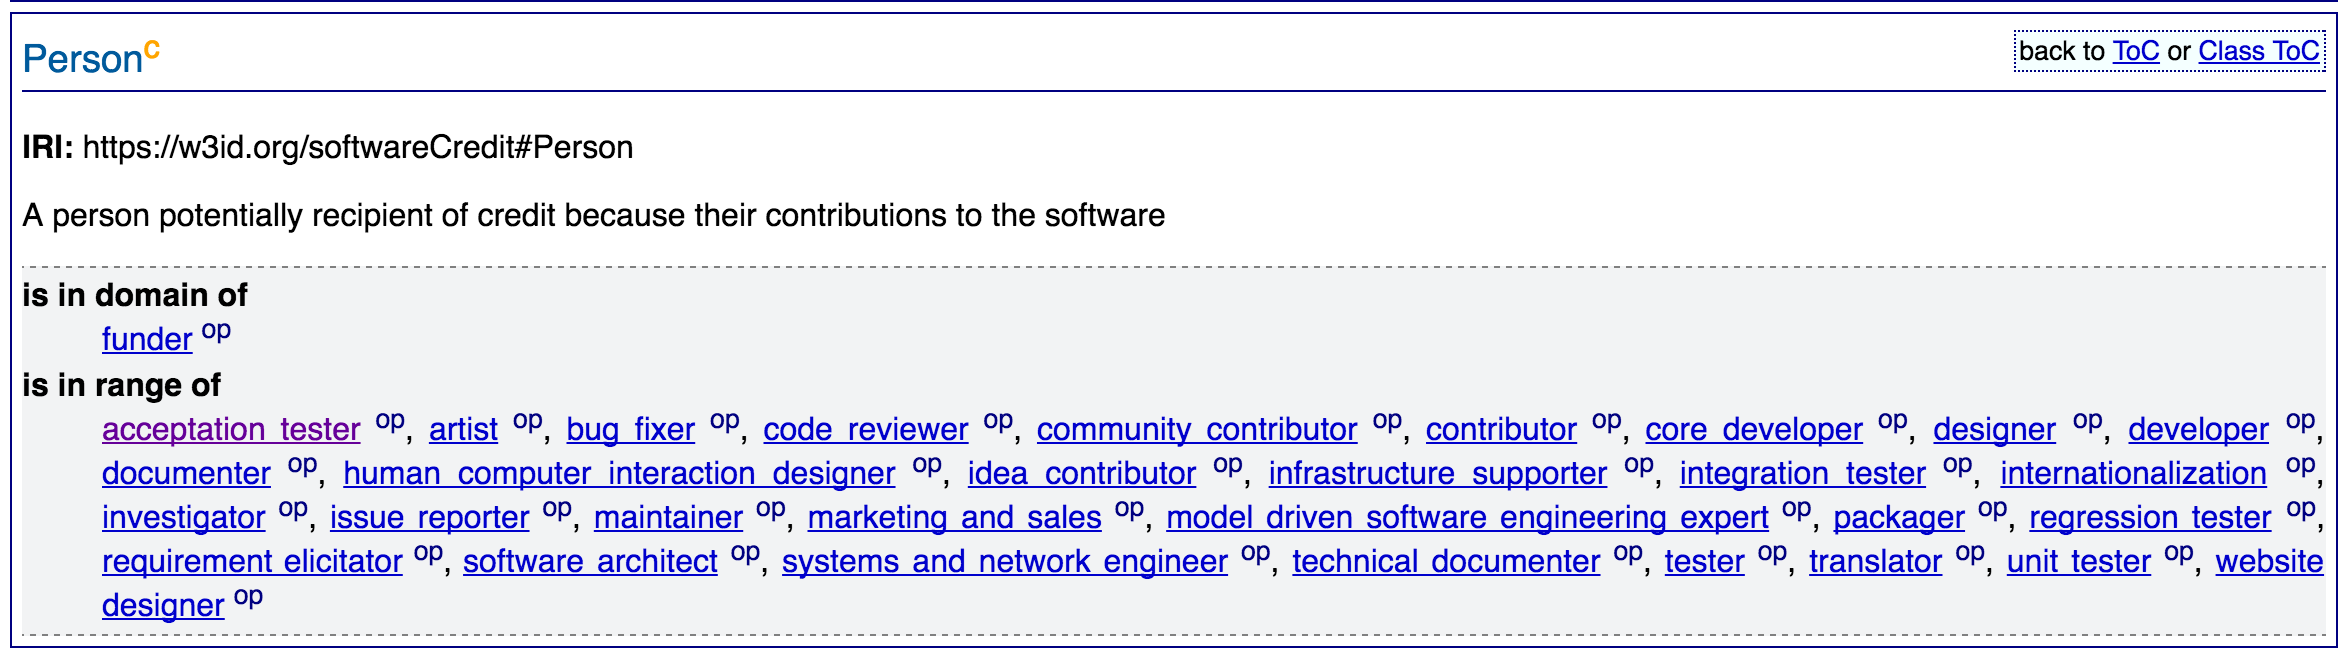
\includegraphics[width=\textwidth]{credits}
\caption{Excerpt from \url{https://w3id.org/softwareCredit} depicting the Person concept with the different roles a person could take upon themselves.\label{fig:credits}}
\end{figure}

A beginning was made with brainstorming towards a number of alternative starting points. The first session led to divisions along the lines of the following concepts: intentions of usage,
degree of openness,
funding,
contributors (single person, group, closed/open community),
community (scale, culture, rights, license)
maturity (process),
accessibility/openness,
Openness
Organizational form
Engineering properties
(Code quality,
Test coverage,
Benchmarking,
Release management,
Semantic versioning,
other metrics
).

\begin{figure}[t]
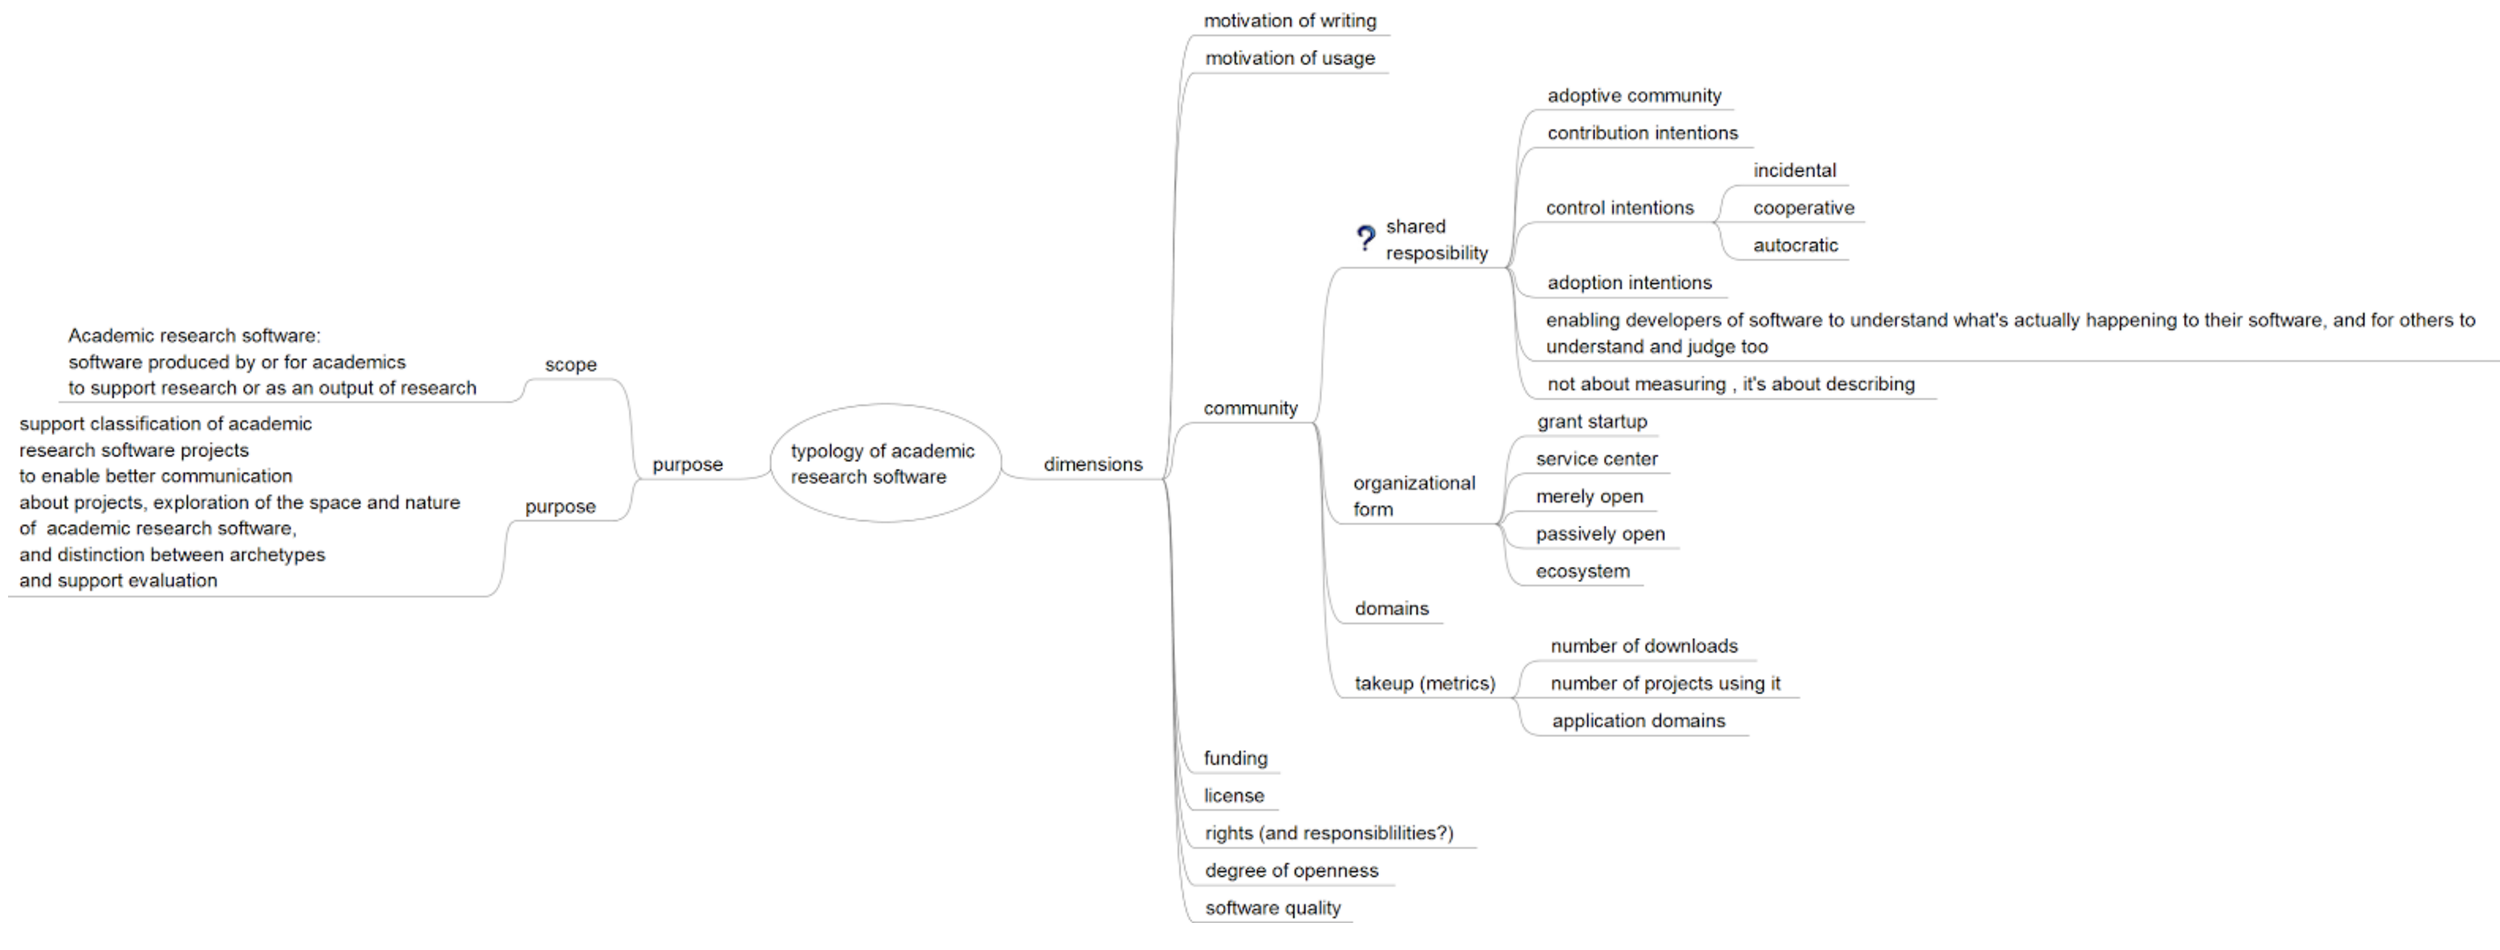
\includegraphics[width=\textwidth]{ontologymap}
\caption{A mindmap of a brainstorm towards an academic software project typology.\label{fig:ontologymap}}
\end{figure}
The second brainstorm resulted in the comparable mindmap depicted in Figure~\ref{fig:ontologymap}.


The final discussion produced a faceted classification with yet different distinctions mainly focused on purpose, intentions and motivations. This finally resulted in a questionnaire (shaped as an online spreadsheet at \url{https://goo.gl/ud5Ik2}) which we filled in for a few dozen projects to see if the distinctions would generate a meaningful overview of typical academic software projects.

The resulting material produced enough to start working on a common paper on the topic. It is important to understand what we are talking about exactly when describing, analyzing and trying to improve academic software projects. It must be noted that clear classifications of software projects in general are not commonplace.


%------------------------------------------------------------------------
\abstracttitle{Empirical Study of Software in Conferences}
\abstractauthor{Jeffrey Carver, James Howison, Robert Haines, Caroline Jay, Kevin Crowston, Oscar Nierstrasz}

The goal of this group was to explore the possibility of carrying out an empirical study to better understand \emph{what software is cited in academic conferences in a particular domain}, how such software is cited, and what are common software practices in that domain.

The group mainly focused on identifying (i) potential \emph{research questions} to be addressed, and (ii) \emph{procedural questions} concerning the logistics of carrying out such a study.

Some of the specific research questions considered were:
\begin{itemize}
\item Which software ends up being mentioned in papers?
\item Who are the developers? (PhD students? Research Software Engineers?)
\item What happens to software after the paper is published?
\item What software engineering practices are applied? (Version control? Testing?)
\item Who pays for software development?
\item What problematic issues commonly arise?
\item What recommendations would improve the quality of software in the fields?
\end{itemize}

Procedural questions included:
\begin{itemize}
\item How to achieve variance? (Do you code for research questions? Venues? Should a grounded approach be used or should predefined hypotheses be considered?)
\item Would machine learning help to classify software in papers?
\item How to start? (Which domain to select?)
\end{itemize}

Katy Huff notes that the Berkeley Institute for Data Science (BIDS, with collaboration from the UW eScience Institute and the NYU center for data science) has collected over 30 case studies from scientists from various domains, synthesized them into lessons learned, and compiled them into a book to be published in 2016 by the University of California Press.\footnote{\url{https://github.com/BIDS/repro-case-studies}}

% It will be published some time this year. The second edition, concerning social science, is currently seeking submissions:  (http://badhessian.org/2016/04/call-for-reproducibility-workflows/, https://bids.berkeley.edu/news/call-reproducibility-workflows )


%------------------------------------------------------------------------
\abstracttitle{Examining Sustainability for a Particular Project}
% \abstractauthor{James Howison, Carole Goble}
\abstractauthor{Carole Goble, Katie Kuksenok, Christoph Becker, Daniel Garijo, Mike Croucher, Dan Katz}


%:TODO -- Examining Sustainability for a Particular Project

%\on{notes extracted from the shared document}
%
%\del{Sustainability of what? Software; service; community; research group!
%Does it make sense to talk about sustainability of software divorced from the sustainability of the team? No.
%%
%- To produce sustainable software you need to sustain the team that produces it.
%- But this can be a distributed team, and it can change over time, it doesn't mean that you have to sustain the original author(s)
%- Does it make sense to talk about sustainability of software divorced from the sustainability of the team? Some think yes, some say No.
%%
%CB: I will venture to say they are entangled - you can say very little about the technical sustainability of a software system alone without considering the social system, etc.; it?s a socio-technical system after all
%DSK: agreed, but it's a complex socio-technical system with lots of moving parts (sometimes called people)
%%
%%
%%
%An example of sustainability debt is the work needed to make the code more modular and more capable of having plug-in components developed
%%
%%
%- Enabling users to get funding for them so they partner with us to make the software. Indirect funding may be achieved this way
%%
%%
%Challenging scenario to conduct an analysis of sustainability debt for specific system in short time since there are multiple, interlinked systems, services, communities, stakeholder groups.
%%
%Carole wants to get large projects, funders, publishers, institutions to support for (subsidize) the software, the service, and the community, so that she can support the long tail of users
%}

\emph{Sustainability} refers to the capacity of a system to endure over time. In the case of software this means that it must continue to be available in the future, on new platforms and meeting new needs.

This breakout group discussed various aspects of sustainability of scientific software:
How can we ensure sustainability of scientific software? What does this mean for a particular project? Does it make sense to talk about sustainability of software divorced from the sustainability of the team?

To produce sustainable software requires sustaining the project organization ---or at least ``a'' project organization--- which produces and maintains the software. With a project we mean an (evolving) team of people and their organization.
Sustainability of the software and of an organized group of people who take responsibility for it are clearly entangled, since you can say very little about the technical sustainability of a software system alone without considering the social system. Note that a sustainable team does not imply an immutable team: a sustainable team can grow or shrink, distribute and swap out team members or leadership in the long term.

A key factor related to software sustainability is \emph{technical debt}, \ie technical shortcuts to achieve a short-term goal that impact long-term quality and maintainability.
An example of investment needed to pay off this debt is the effort required to make the code more modular and more amenable to accepting new plug-in components.
A challenging scenario would be to conduct an analysis of sustainability debt for specific systems in a short time since there are multiple, interlinked systems, services, communities, and stakeholder groups.

A recurring problem is the issue of obtaining funding to maintain scientific software and guarantee its sustainability for the community and the long tail of users.


%------------------------------------------------------------------------
\abstracttitle{Making the Impact of Software more Visible}
\abstractauthor{Matthew Vaughn, Katy Huff, Matt Turk, Rob van Nieuwpoort, Alice Allen, Andrei Chi\c{s}, Cecilia Aragon, Claude Kirchner, Dan Katz}

A fundamental problem in selected scientific fields, such as physics and astronomy, is that a huge amount of effort is invested in producing scientific software, but only published papers count towards scientists' careers. This leads inevitably to the process, ``I write the software and then I write a paper to get credit.'' We need a cultural change in the scientific community to raise awareness that scientific software itself represents valuable intellectual content and scientific innovation directly and explicitly.

This breakout group discussed the status quo and ways to change it. Journals exist in Computer Science and Bio-Informatics that are home to intellectual contributions of software packages. Several computer science conferences explicitly support ``artifact evaluation'' where software contributions are scrutinized and appreciated as part of the academic review process. But the appreciation of software as academic output does not seem to be universal across domains.

Appreciation for software seems more natural in Computer Science, which explains recent efforts in this field to making the impact of software visible, yet across the board the field is not particularly ahead in this regard with respect to other fields. An important positive factor is the recent focus in research towards ``innovation'' and ``valorization'' which puts tangible and transferable results of Computer Science in the form of working software in the spotlight. Bio-Informatics though, is ahead of the pack, which may be due to its explicit branding as a the informatics branch of Biology.

One critical need that was identified is to explicitly include software output into the evaluation processes of both academics and academic institutions. Currently, publishing software may give you a DOI (\eg via Zenodo\footnote{\url{https://zenodo.org/}}) but this neither brings you reputation nor does it contribute to a positive evaluation per se, unless this DOI is indexed as part of your records and citations to it are credited to your metrics.
% ON: "per se" is Latin, so no accent is needed
Problems with making software output part of the academic process were discussed. For example, software lasts longer than the citable snapshots we have now, leading to evolving author lists and evolution between software versions, which may in turn lead to software growing far beyond the original scope. Short papers about software are too short to make the academic challenges and contributions observable, while long papers about software hide the software contributions under the traditional paper-style contributions. And finally, reading and appreciating source code is just hard especially if it is not originally written with such an audience in mind.

Several possible solutions were discussed: %\jv{based on the notes, but I did use some imagination here:}
\begin{itemize}
	\item Papers could capture more about the software's intellectual impact; \ie in a separate section akin to the standard ``research method'' and ``threats to validity'' sections.
    \item Letters of support may be the best way to communicate software impact to tenure committees.\footnote{This has been the case in Computer Science in the US for about 20 years, due to a National Research Council report~\cite{NRC-CS-1994} that is frequently quoted in such letters.}
    \item People could claim their contributions more explicitly:
    	web pages are needed to document software contributions;
		research software engineers should be motivated to co-author papers;
		and scientists who develop software must be willing to be proud and certainly unapologetic about their software contributions in front of tenure committees.
    \item Rubrics and templates for letters of recommendation should be developed to highlight intellectual contributions from code.
    \item A Research Coordination Network (RCN) workshop\footnote{RCNs are an NSF instrument: \url{https://www.nsf.gov/funding/pgm_summ.jsp?pims_id=11691}. Presumably similar instruments exist in other countries.} should be started to showcase intellectual content for academic software.
    \item Encourage the formation of a prestigious scientific software award.
\end{itemize}

%------------------------------------------------------------------------
\abstracttitle{Reviewing FORCE11 Software Citation Principles}
\abstractauthor{Dan Katz, Robert Haines, James Howison, Katy Huff, Caroline Jay, Matt Vaughn}

This group came together to contribute to the FORCE11 software citation principles. The FORCE11 website\footnote{\url{https://www.force11.org/software-citation-principles}} says: ``Based on a review of existing community practices, the goal of [FORCE11] was to produce a consolidated set of citation principles that may encourage broad adoption of a consistent policy for software citation across disciplines and venues.''

The breakout group reviewed the different personas (roles) in relation to the software citation principles to see if their interests were reflected appropriately:
reviewer, author of software, designer of citation style, reader of paper, user of software, funding agency, publisher.

This review was passed on to the FORCE11 Software Citation Working Group editors, leading to updates to the citation principles where these were deemed necessary, and the final version was recently published~\cite{10.7717/peerj-cs.86}, including these updates.


%------------------------------------------------------------------------
\abstracttitle{Future Research directions}
\abstractauthor{Claude Kirchner, James Williams, Oscar Nierstrasz, Katie Kuksenok, Jurgen Vinju, Benoit Combemale, Matt Vaughn, Cecilia Aragon, Alice Allen \jv{based on email exchange so far, could be people missing or extra}}

This breakout group discussed a number of possible themes for future research projects or initiatives.
Of the topics discussed the following ones were elaborated in enough detail to be included as part of the Dagstuhl Manifesto:

\begin{enumerate}
\item \emph{Quantifying the availability of scientific software:} this research would attempt to determine how research software exists, for which domains is it developed, who owns it, who pays for it, who maintains it. The research would also attempt to identify opportunities for reuse, sharing, and collaboration.

\item \emph{Facilitating software discovery within and across disciplines:} the key research question here is to determine, aside from standards, what other approaches can effectively support discoverability of available research software.

\item \emph{Sustainability of software experimentation:} how can we ensure reproducibility of software experiments, not just in the short or medium term, but in the very long term?

\item \emph{Software engineering tools improving productivity by tailoring to intent and skill:} not all research software requires the same development rigor and discipline as commercial software, yet all would benefit from from skills beyond that of ``hobbyist'' programmers. How can we appropriately select and adapt the level of software engineering discipline appropriate to a given research project?

\item \emph{Re-tooling the bibliographic software toolchain for software citation:} existing bibliographic tools are highly tailored towards academic writing. How do we adapt the metadata and tools to get the right meta-information about software into citations?

\item \emph{Analysis of scientific software ecosystem metadata:} how can we effectively monitor and analyze metadata about research software in the large?

\end{enumerate}


%------------------------------------------------------------------------
\abstracttitle{Design of the Manifesto}
\abstractauthor{Claude Kirchner, Oscar Nierstrasz, James Howison, Katie Kuksenok, Jurgen Vinju}

A key goal of this Dagstuhl Perspectives Workshop has been to produce a \emph{Dagstuhl Manifesto}\footnote{Dagstuhl Perspectives Workshops explore new and emerging topics in Computer Science, and are expected to produce \emph{Dagstuhl Manifestos} that capture trends and developments related to these topics. See: \url{http://www.dagstuhl.de/en/publications/dagstuhl-manifestos/}} to serve as a roadmap towards future professional software engineering for software-based research instruments and other software produced and used in an academic context.

Throughout the week, each of the breakout groups logged their discussions in a common, shared Google document, and took care to identify specific ``pledges'' that could serve as input to the manifesto. The goal was to ensure actionable outcomes which called on individuals themselves to act, rather than to ask others to act on their behalf. This intent acknowledges that ``we'' are the community and that visible action provides ``social proof'' and motivates others. The pledges were based on a template: (i) the pledge itself, expressed in the form ``I will \emph{take some specific actions to support EAS}'', (ii) \emph{background} motivating the pledge, (iii) \emph{contradictions or concerns} that could impact the pledge, (iv) specific \emph{actions needed}, and (v) identification of other \emph{players who need to act}.

By the end of the week, some 30-odd candidate pledges had been collected for the manifesto.
The manifesto design breakout group then set out to cluster the pledges around common, overarching themes, namely:
(i) Citation \& Reviewing;
(ii) Recognition;
(iii) Making intellectual content visible;
(iv) Software Projects; and
(v) Sustainability.

In a subsequent session, the group pared down the list of candidates, eliminating seemingly redundant or confusing pledges, and pledges lacking substantial description, yielding 18 surviving candidates.

Subsequent to the termination of the workshop, a poll was prepared to rank these 18 pledges. The list was subsequently simplified and reduced to 5 key pledges in three categories: (i) Citation, (ii) Careers, and (iii) Development.
(The poll has also been run at WSSSPE 2016, though the results have not yet been analyzed.)

At the time of the preparation of this report, a draft manifesto is under preparation as a GitHub project.\footnote{\url{https://github.com/DagstuhlEAS/draft-manifesto}}


%% ==================================================
%\section{Research questions}
%
%\on{From the manifesto?}

% \bibliographystyle{plain} % ON: already at top
\bibliography{report}
\end{document}
